\chapter{User Documentation}\label{chapter:user}

\begin{figure}[htbp]
    \centering
    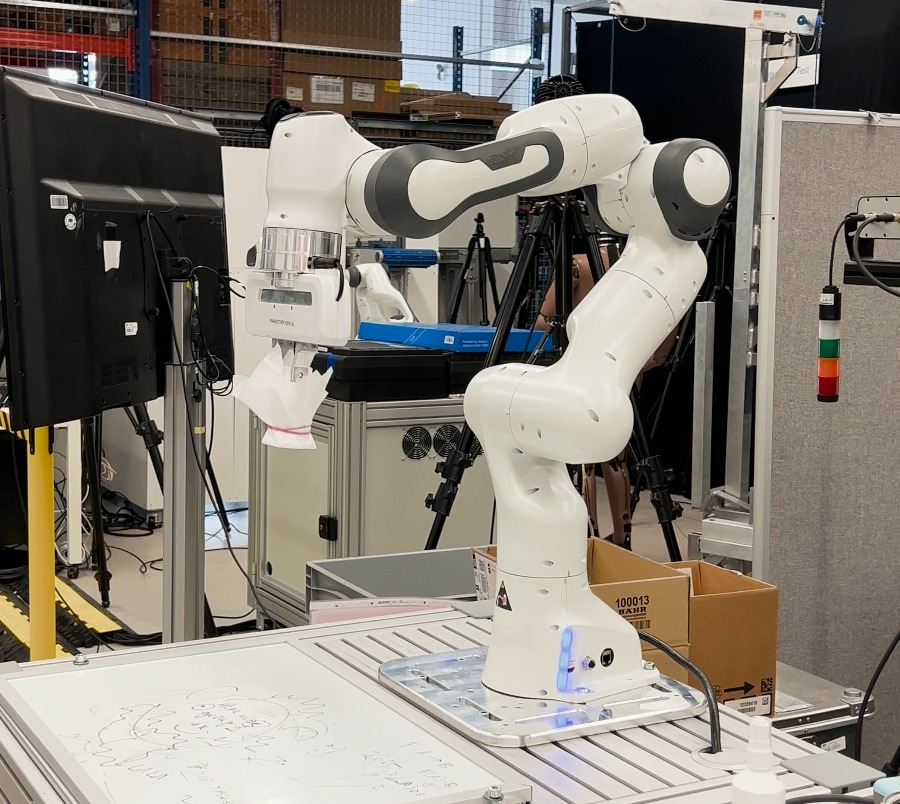
\includegraphics[width=0.5\linewidth]{figures/franka-example.png}
    \caption{Franka Emika Panda Robot}
    \label{fig:franka-example}
\end{figure}

In this chapter it will be explained how to build and execute the program with the real Franka Robot. Keep in mind that without physical source, you would need to address Developer Documentation to run it using simulator. You can see the example of Franka robot \autoref{fig:franka-example}


\section{Installation and Usage}
The following installation was partially taken from our supervisor \copyright \href{https://alessandromelone.github.io/}{Alessandro Melone} \href{mailto:alessandro.melone@tum.de}{alessandro.melone@tum.de}

\subsection{Cloning}
First clone the repo to your local machine
\begin{lstlisting}[language=bash]
git clone https://gitlab.lrz.de/tum-impl-ss24/assignment2-group1
git checkout main
\end{lstlisting}

\subsection{Setup}
To use properly the docker you need modify the \texttt{.env} file replacing
\begin{itemize}
    \item \texttt{<username>} with your username (i.e., the output of \texttt{whoami} in your terminal) in \texttt{USERNAME=<username>}
    \item \texttt{<username>} with your username in \texttt{ROS\_WS=/home/<username>/ros\_ws}, (\texttt{ROS\_WS} will be the path of your ROS2 workspace in the container)
    %   
\end{itemize}

\begin{quote}
Reason: these variables are used to setup the container user with same credential of the host (by default the container would run as superuser). Among several benefits, this implies that all the files generated by the container have the same ownership of the one generated by the host. For further info, refer to this \href{https://github.com/joemccann/dillinger}{guide}.
\end{quote}

\subsection{Usage}
At the first usage, build the docker image using the following command in the project folder:
\begin{lstlisting}[language=bash]
./setup_docker.bash
\end{lstlisting}

After, open a terminal in the project folder and run:
\begin{lstlisting}[language=bash]
docker compose up
\end{lstlisting}

Now a docker container is running on your machine. To access the container, open another terminal and run:
\begin{lstlisting}[language=bash]
docker compose exec -it gazebo_franka_ros1-ros1_node-1 bash
\end{lstlisting}

\begin{quote}
this is the equivalent of opening a terminal on your Ubuntu installation but on the Ubuntu installation running in the container.
\end{quote}

where \texttt{gazebo\_franka\_ros1-ros1\_node-1} is the name of the container you want to access. To see the names of all the containers running on your machine, you can use \texttt{docker ps}.

\subsection{First Usage and Build}
Access a running container and use the following command to initialize your \texttt{catkin\_ws}:

\begin{enumerate}
    \item Inside container of \textbf{terminal1} run 
        \begin{lstlisting}
            catkin_make    
        \end{lstlisting}
    \item Open \textbf{terminal2} and run 
        \begin{lstlisting}
            roslaunch trajectory_gen cartesian_impedance_example_controller.launch
            \\ robot:=panda robot_ip:=192.168.3.8
        \end{lstlisting}
        This will connect your code from franka-ros to the remote Franka robot
    \item Open new \textbf{terminal3} and remove other publishers, if there are any
        \begin{lstlisting}
            rosnode kill /interactive_marker
        \end{lstlisting}
    \item Go back to the \textbf{terminal1} and run 
        \begin{lstlisting}
            rosrun trajectory_gen trajectory_gen_node
        \end{lstlisting}
    \end{enumerate}




\section{Operation Demo}

Here are some images showcasing how the robot moves

\begin{figure}[htbp]
    \centering
    \begin{subfigure}{0.45\textwidth}
        \centering
        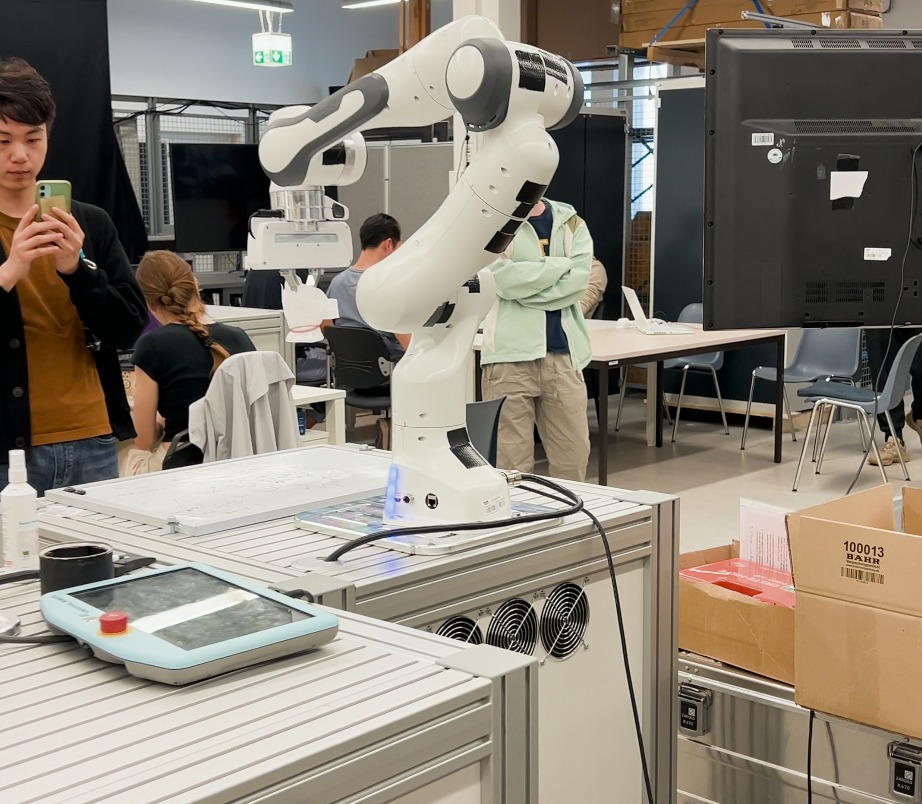
\includegraphics[width=\textwidth]{figures/start-pos-robot.png}
        \caption{Linear movement towards the surface}
        \label{fig:franka-down}
    \end{subfigure}
    \hfill
    \begin{subfigure}{0.45\textwidth}
        \centering
        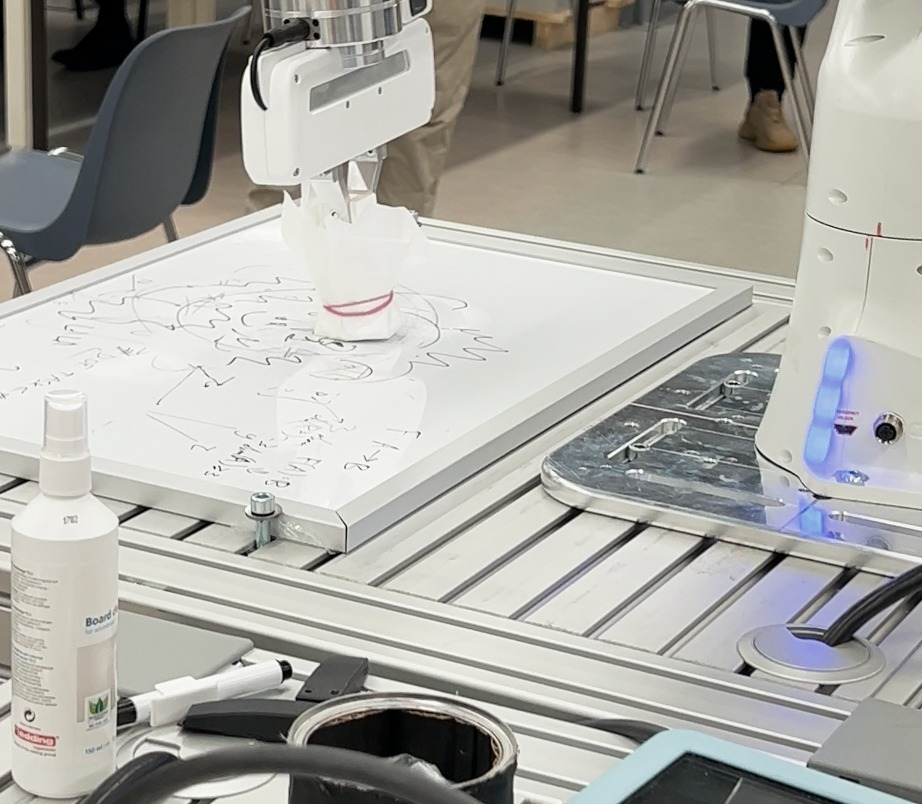
\includegraphics[width=\textwidth]{figures/middle-pos-robot.png}
        \caption{Rotational movement on the surface}
        \label{fig:franka-mid}
    \end{subfigure}

    \begin{subfigure}{0.45\textwidth}
        \centering
        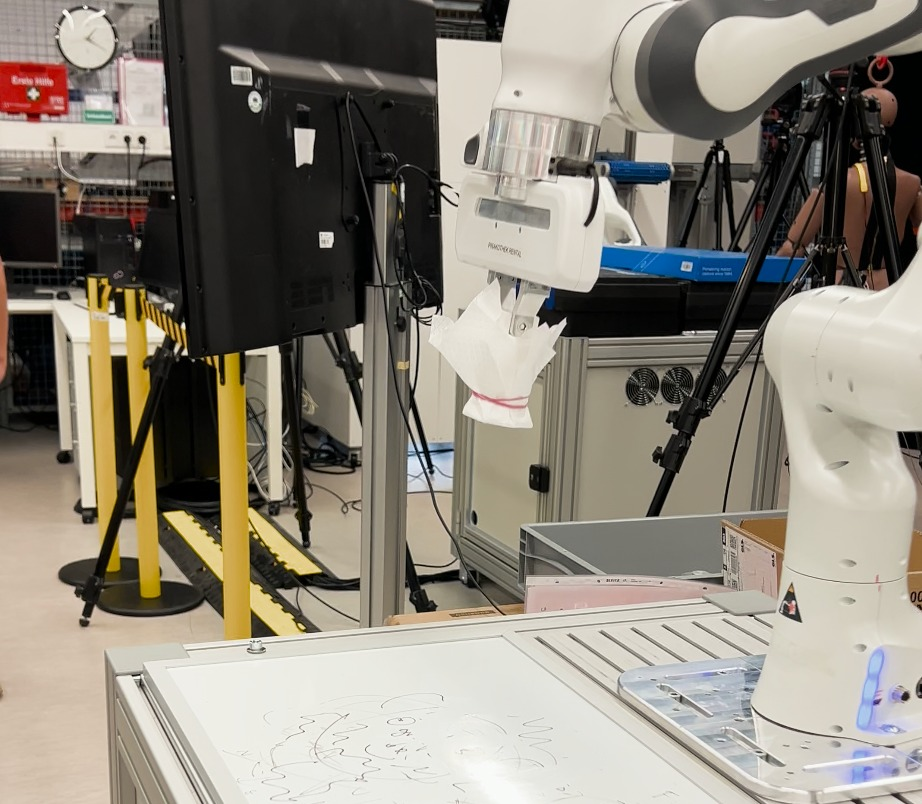
\includegraphics[width=\textwidth]{figures/up-pos-robot.png}
        \caption{Going up to initial position}
        \label{fig:franka-up}
    \end{subfigure}
    \hfill
    \begin{subfigure}{0.45\textwidth}
        \centering
        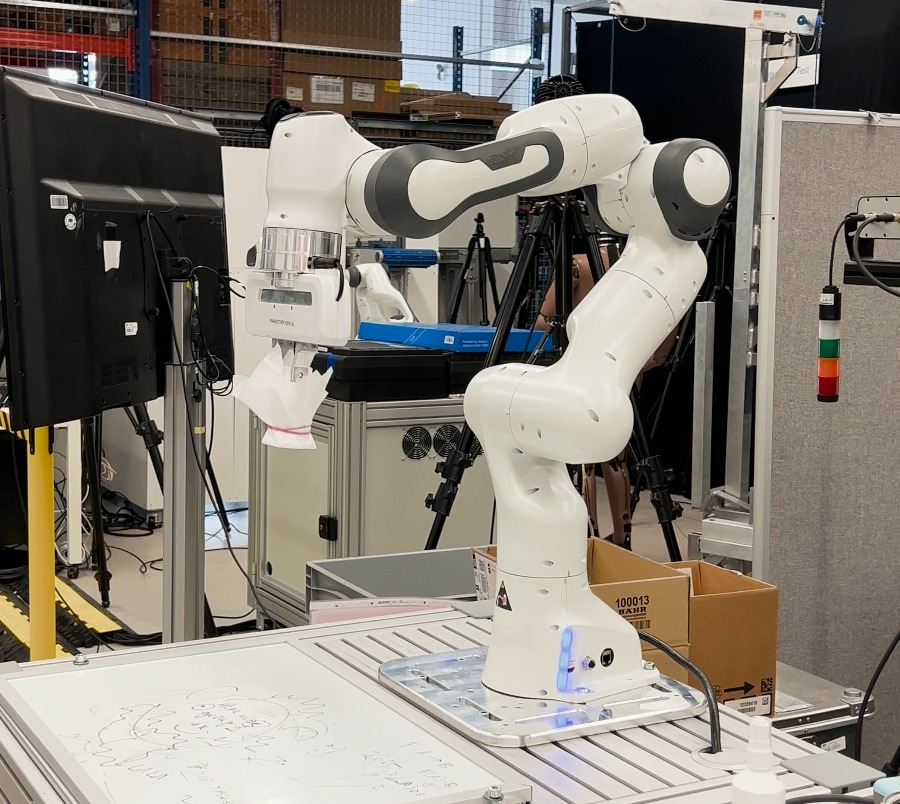
\includegraphics[width=\textwidth]{figures/initial-pos-robot.png}
        \caption{Return to initial robot position}
        \label{fig:franka-init}
    \end{subfigure}

    \caption{Different states of Franka movement during program execution}
    \label{fig:franka-grid}
\end{figure}
